\chapter{Introduction}
\section{Background and research purpose}
In the foreseeable future, the electrification of ocean systems, renewable ocean power sources and ocean energy networks will be necessary, which could help accelerate the growth and deployment of ocean renewable energy and ways to explore and understand the ocean \cite{Orekan}. To realize electrification in the ocean requires good water resistance, durability and long-distance remoteness. For the waterproofness of the equipment, we can use high-performance waterproof and pressure-resistant materials. The durability of electrical equipment requires low-consumption AUV and high-energy batteries or continuous energy supply for the equipment. Long-distance maneuverability needs to solve the problem of long-distance underwater communication. We can use xx to reach xxkm underwater long-distance distance.
Certain attributes of ocean energy, such as its high energy density, make it attractive as a grid-connected energy, or it may make it an isolated and remote ocean energy, thereby providing power solutions for the sustainable development of ocean space, which is attractive. The rapid development of distributed ocean energy applications (such as underwater sensor networks, ocean sensors and monitoring technologies, ocean automatic network buoys, and deep sea and tsunami buoys) is advantageous. In particular, it can power an autonomous underwater vehicle (AUV) whose service life is limited by its battery power.

\begin{figure}[htbp]
    \centering
    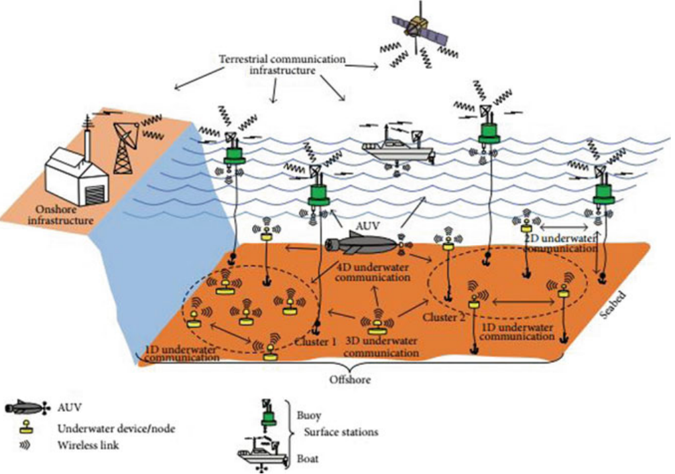
\includegraphics[width=0.9\linewidth]{images/1_underwater_sensor_networks.png}
    \caption{Underwater sensor networks architecture \cite{Nayyar}.}
\end{figure}

% \begin{figure}[htbp]
%     \centering
%     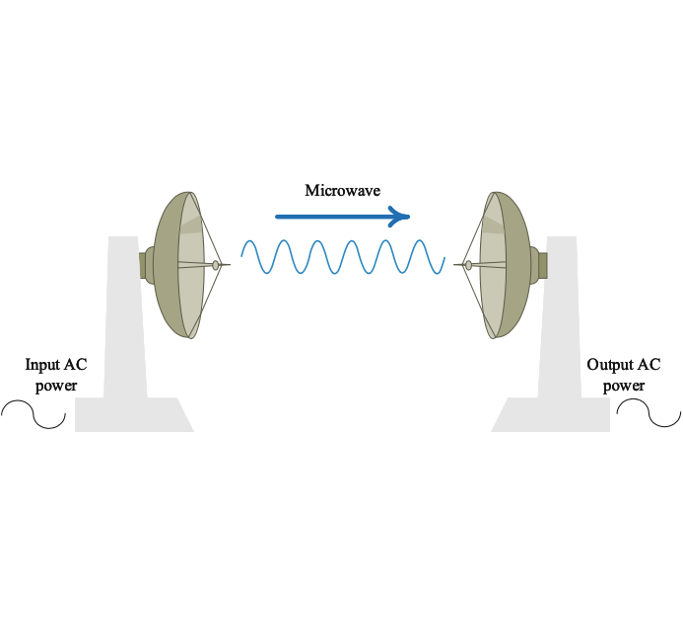
\includegraphics[width=150pt]{images/1_microwave_power_transfer.png}
%     \caption{Microwave power transfer.}
% \end{figure}
% \begin{figure}[htbp]
%     \centering
%     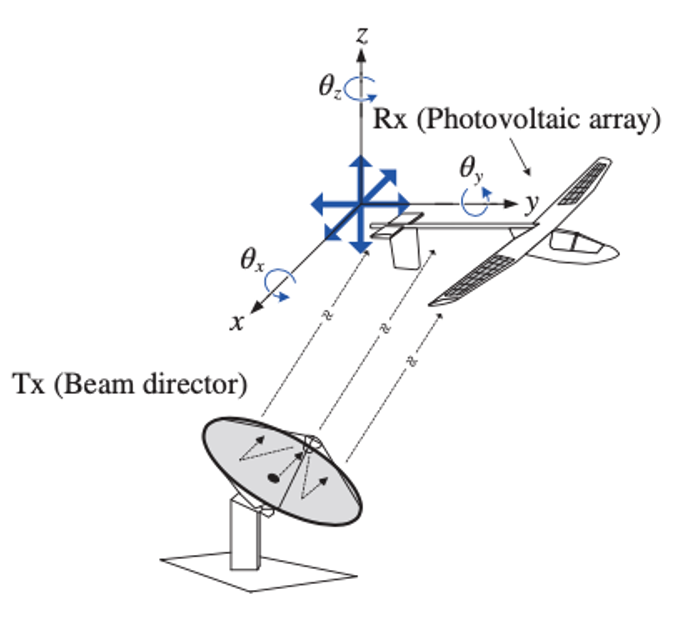
\includegraphics[width=150pt]{images/1_laser_power_transfer.png}
%     \caption{Laser power transfer.}
% \end{figure}


\section{Wireless power transfer technologies}

Far field power transfer
\begin{figure}[htbp]
    \begin{subfigure}{0.5\textwidth}
        \centering
        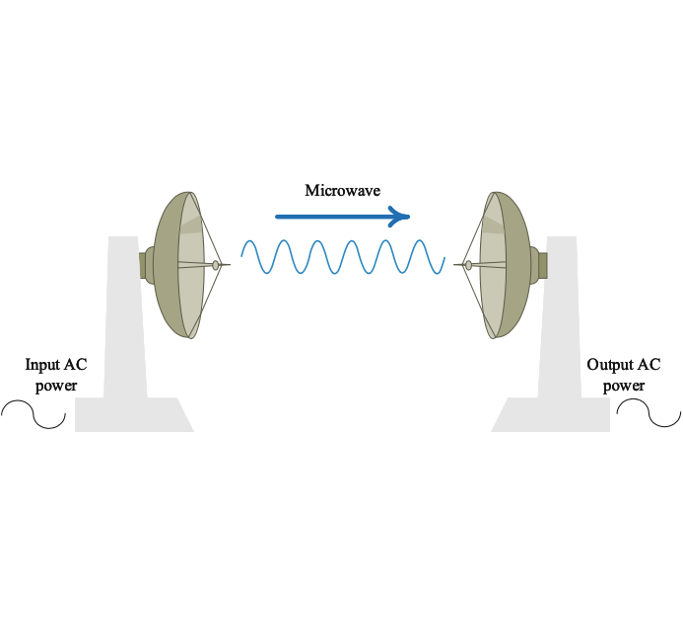
\includegraphics[width=0.9\linewidth]{images/1_microwave_power_transfer.png}
        \caption{Microwave power transfer \cite{Orekan}.}
        \label{fig:subim1}
    \end{subfigure}
    \begin{subfigure}{0.5\textwidth}
        \centering
        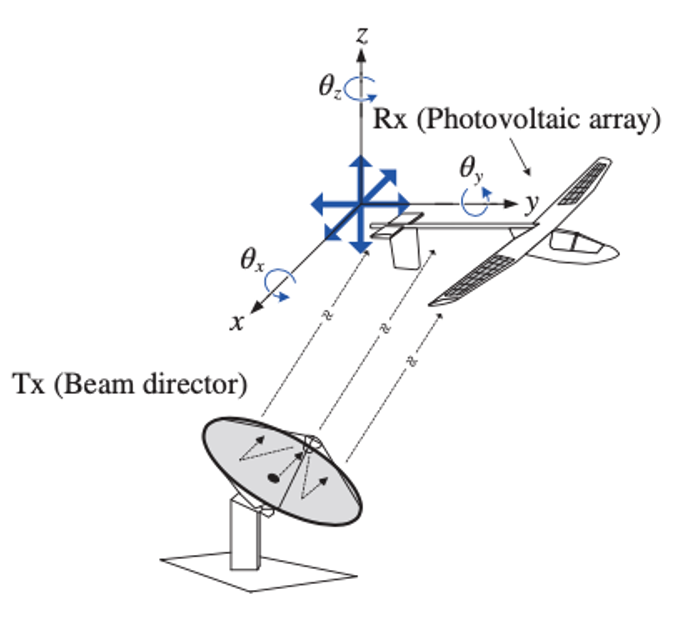
\includegraphics[width=0.9\linewidth]{images/1_laser_power_transfer.png}
        \caption{Laser power transfer \cite{Chun}.}
        \label{fig:subim2}
    \end{subfigure}

    \caption{Far-field wireless power transfer.}
    \label{fig:image2}
\end{figure}

\begin{figure}[htbp]
    \begin{subfigure}{0.5\textwidth}
        \centering
        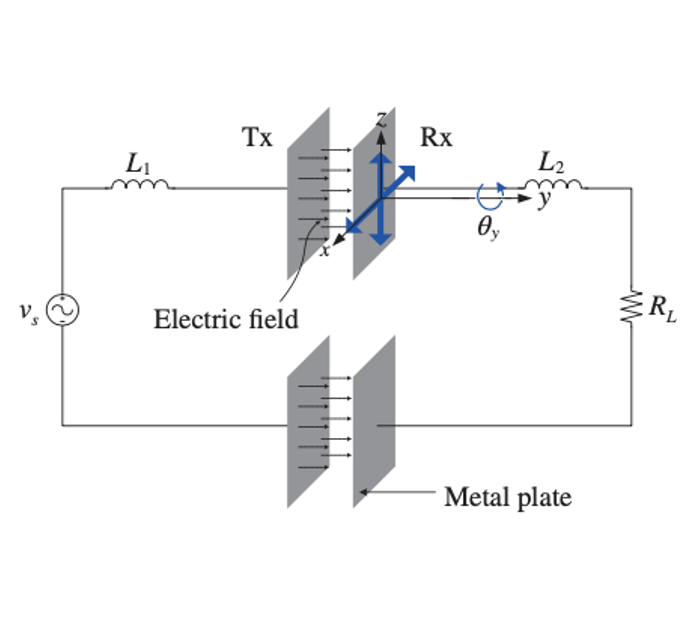
\includegraphics[width=0.9\linewidth]{images/1_capacitive_power_transfer.png}
        \caption{Capacitive power transfer \cite{Chun}.}
        \label{fig:subim1}
    \end{subfigure}
    \begin{subfigure}{0.5\textwidth}
        \centering
        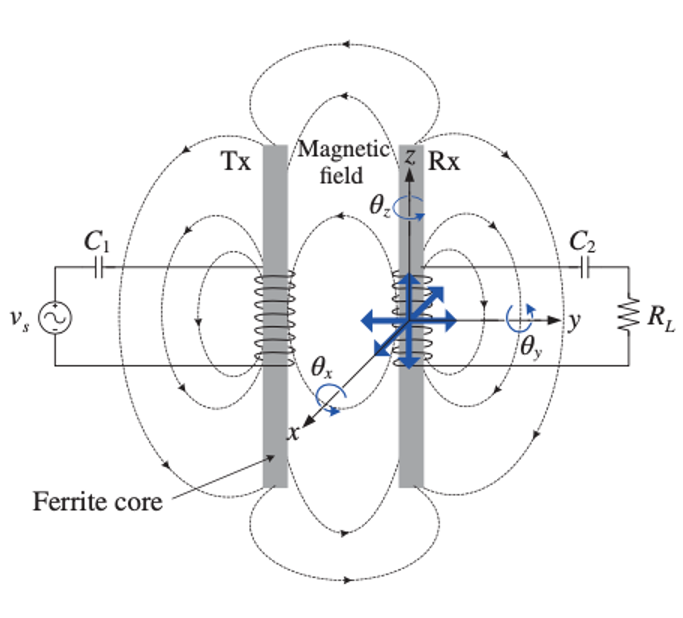
\includegraphics[width=0.9\linewidth]{images/1_inductive_power_transfer.png}
        \caption{Inductive power transfer \cite{Chun}.}
        \label{fig:subim2}
    \end{subfigure}

    \caption{Near-field wireless power transfer.}
    \label{fig:image2}
\end{figure}

\makeatletter
\newcommand{\thickhline}{%
\noalign {\ifnum 0=`}\fi \hrule height 1pt
    \futurelet \reserved@a \@xhline
}
\newcolumntype{"}{@{\hskip\tabcolsep\vrule width 1pt\hskip\tabcolsep}}
\makeatother

\begin{table}[h!]
    \centering
    \begin{tabular}{ |c|c|c|m{3.5cm}<{\centering}|m{3.5cm}<{\centering}| }
        % \thickhline
        \hline
        \textbf{Technology} & \textbf{Range} & \textbf{Frequency}         & \textbf{Antenna devices}                    & \textbf{Applications}                             \\\hline
        % \thickhline
Microwaves          & hm - km        & GHz                        & Parabolic dishes, phased arrays, rectennas  & Satellite, Drone aircraft                         \\ \hline
Optical             & dam - km
                    & $\geq$THz      & Lasers, photocells, lenses & Drone aircraft, Space elevator                                                                  \\ \hline
Capacitive          & cm - m         & kHz – MHz                  & Metal plate electrodes                      & Smartcards, Biomedical implant
\\ \hline
Inductive           & mm - m         & Hz – GHz                   & Tuned wire coils, lumped element resonators & Electric toothbrush, Smartphone, Electric vehicle
\\ \hline
    \end{tabular}
    \caption{The different wireless power technologies.}

\end{table}

\section{Underwater wireless power transfer}



\section{The main research content of this thesis}

\section{Roadmap}